% To produce pdf under linux, run
% pdflatex hw3.tex

% Credit for this template goes to Dr. Jerry Zhu.

\documentclass{article}
\usepackage[margin=1in]{geometry}
\usepackage{amsmath,amssymb}
\usepackage{bbm}
\usepackage{graphicx}
\usepackage{hyperref}
\usepackage{outlines}
\usepackage{enumitem}
\usepackage{float}
\usepackage{xcolor}
\usepackage{parskip}
\usepackage[skip=0.5\baselineskip]{caption}

\def\bfx{\mathbf x}
\def\R{\mathbb R}
\def\E{\mathbb E}
\def\argmax{\mathrm{argmax}}
\def\argmin{\mathrm{argmin}}


\newenvironment{soln}{
	\leavevmode\color{blue}\ignorespaces
}{}



\title{CS760 Spring 2019 Homework 4}
\author{}
\date{}
\begin{document}
\maketitle


%%%%%%%%%%%%%%%%%%%%%%%%%%%%%%%%%%%%%%%%%%%%%%%%%%%%%%%%%%%%%%%%%%%%%%%%%
% Insert your name and email here:

Name: Stewart Kerr

Email: shkerr@wisc.edu 

%%%%%%%%%%%%%%%%%%%%%%%%%%%%%%%%%%%%%%%%%%%%%%%%%%%%%%%%%%%%%%%%%%%%%%%%%


\begin{figure}[h]
\centering
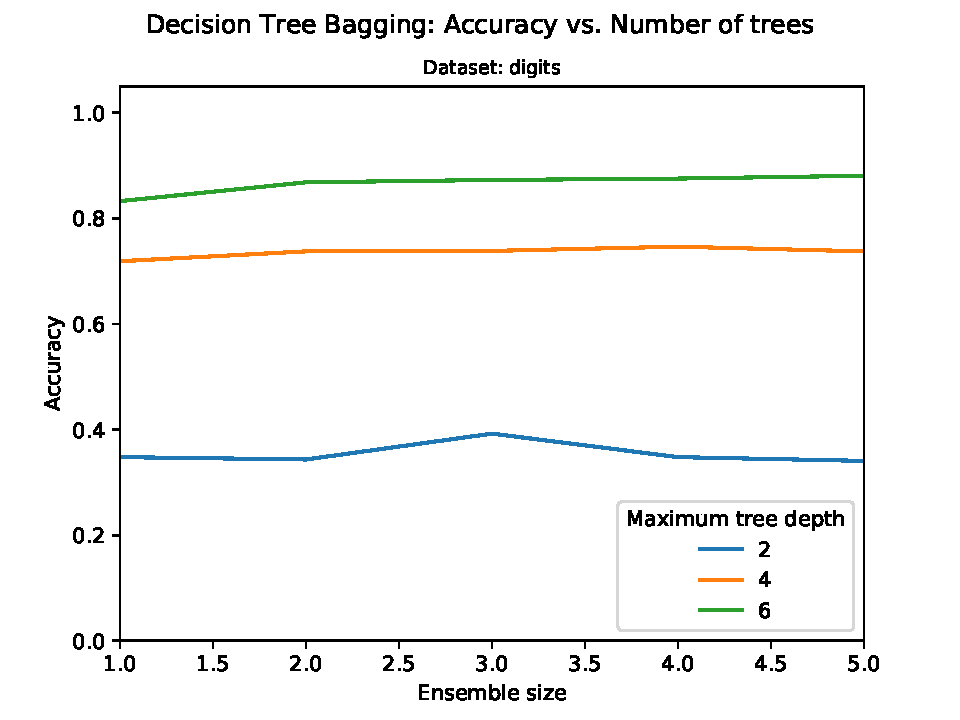
\includegraphics[scale=1]{bagged_tree_plot}
\end{figure}

With bagging, the accuracy directly increases with larger maximum tree depth but does not change much with increasing ensemble size. Bagging is useful to combine classifiers with high variance. In the context of decision trees, these are trees that have a large depth - these trees will have small bias (and thus tend to overfit) but will have high variance between different input data. Bootstrap aggregation helps to decrease this variance such that the overall error is low.

\pagebreak

\begin{figure}[h]
\centering
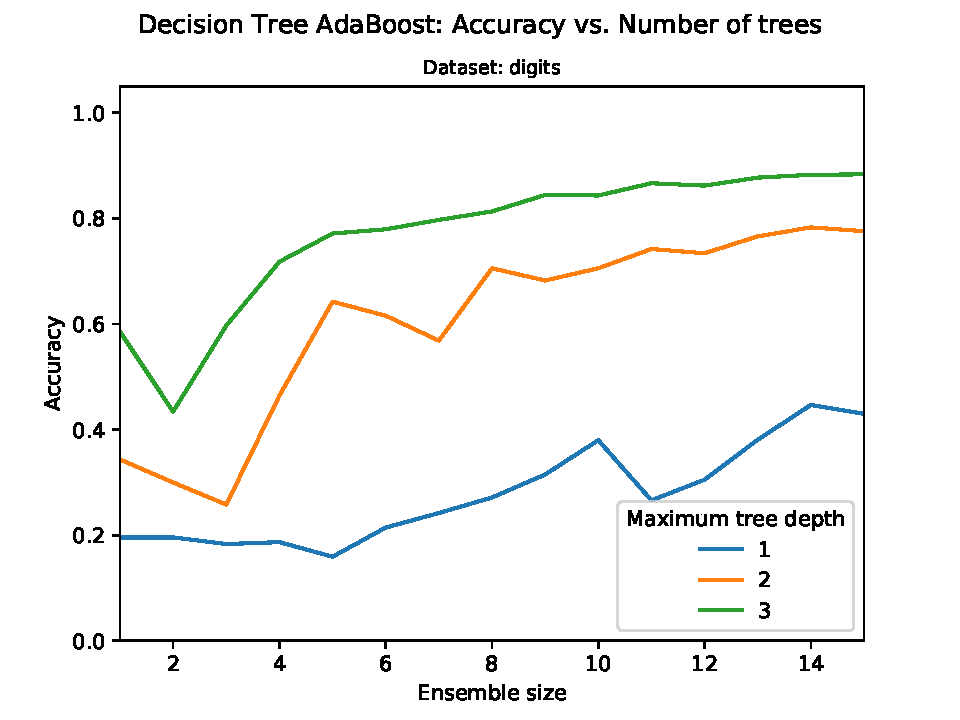
\includegraphics[scale=1]{boosted_tree_plot}
\end{figure}

With Adaboost, we are building successively on previous classifiers. Thus, we can use poor classifiers (that is, decision trees with a small depth - large bias) and still obtain good results by increasing the number of training iterations (ensemble size). From the figure, we've obtained an accuracy over 0.80 using a small tree that has a maximum depth of only three. 

For this particular problem, I think that bagging is a stronger method. Increasing the ensemble size increases computation time much more than increasing maximum tree depth, thus bagging (which does not require a large ensemble size) will run much faster that boosting.

\end{document}
]